%% LaTeX2e class for student theses
%% sections/methodology.tex
%% 
%% Karlsruhe Institute of Technology
%% Institute for Program Structures and Data Organization
%% Chair for Software Design and Quality (SDQ)
%%
%% Dr.-Ing. Erik Burger
%% burger@kit.edu
%%
%% Version 1.3.6, 2022-09-28

\chapter{Methodology}
\label{ch:Methodolody}

%% -------------------
%% | Example content |
%% -------------------
Since our continual learning approach is, to the best of our knowledge, the first approach to combine pool-based active learning with continual
learning, we explain our approach in detail in this chapter as well as the motivation for it. We then transfer our approach to the domain of model
stealing. Because we build upon the framework of ActiveThief, we describe how our approach compares to the original approach in detail.

\section{Continual Active Learning}
\label{sec:Methodology:ContinualActiveLearning}
A major contribution of this thesis is that we combine the two learning paradigms of continual learning and active learning. To motivate the idea of
combining Continual Learning and Active Learning, we will first outline the classic Continual Learning Setting and the classic Active Learning Setting.
Next we explain common issues with these two learning paradigms and how we aim to overcome these by combining both paradigms. Finally, we will give
a detailed description of our approach. 

\subsection{The classic Continual Learning Setting}
\label{sec:Methodology:CLSetting}
%Mention that CL Setting consists of multiple tasks, task can and usually are independent
% Outline classic Continual Learning Workflow with a figure
In the typical continual learning setting, the model is trained on a sequence of tasks. Each task $T_i = {x_k,y_k | k \in \{1,\ldots,n\}}$ is a set of instances 
with their respective label. Together, the tasks form a dataset $D = \bigcup\limits_{i=1}^{N} T_i$. It is important to note that
the distribution of two distinct tasks $P(T_i)$  and $P(T_j) (i \neq j)$ are not necessarily the same. Most often in fact, the tasks are independent of each
other, which is why neural networks struggle to perform well on multiple tasks at once. This also means that the size of two distinct datasets can be
different, i.e. $|T_i| \neq |T_j|$ and so can the number of classes $|{y_k | \exists x_k: x_k,y_k \in T_i}| \neq |{y_l | \exists x_l: x_l,y_l \in T_j}|$.
When training a model on a sequence of tasks, the model is first fed with the data of the first task $T_1$ and then trained on it. After the model has been trained
on the first task, it can either be trained on the next task or deployed to classify samples stemming from the distribution of the first task. Next, the model is
trained on the second task. After being trained on the second task, the model should now be able to classify samples from the distribution of the first task as well
as the second task. This process is repeated until the model has been trained on all tasks. After being trained on all tasks, the model should be able to classify
%samples following the distribution of all the tasks it was trained on. This workflow is illustrated in Figure \ref{fig:CLWorkflow}. \\
The main difference between the continual learning setting and classic machine learning is that in the classic machine learning setting, the model is never retrained
once it is deployed. In the continual learning setting however, the model is retrained whenever a new task arrives.

\begin{figure}[ht]
    \centering
    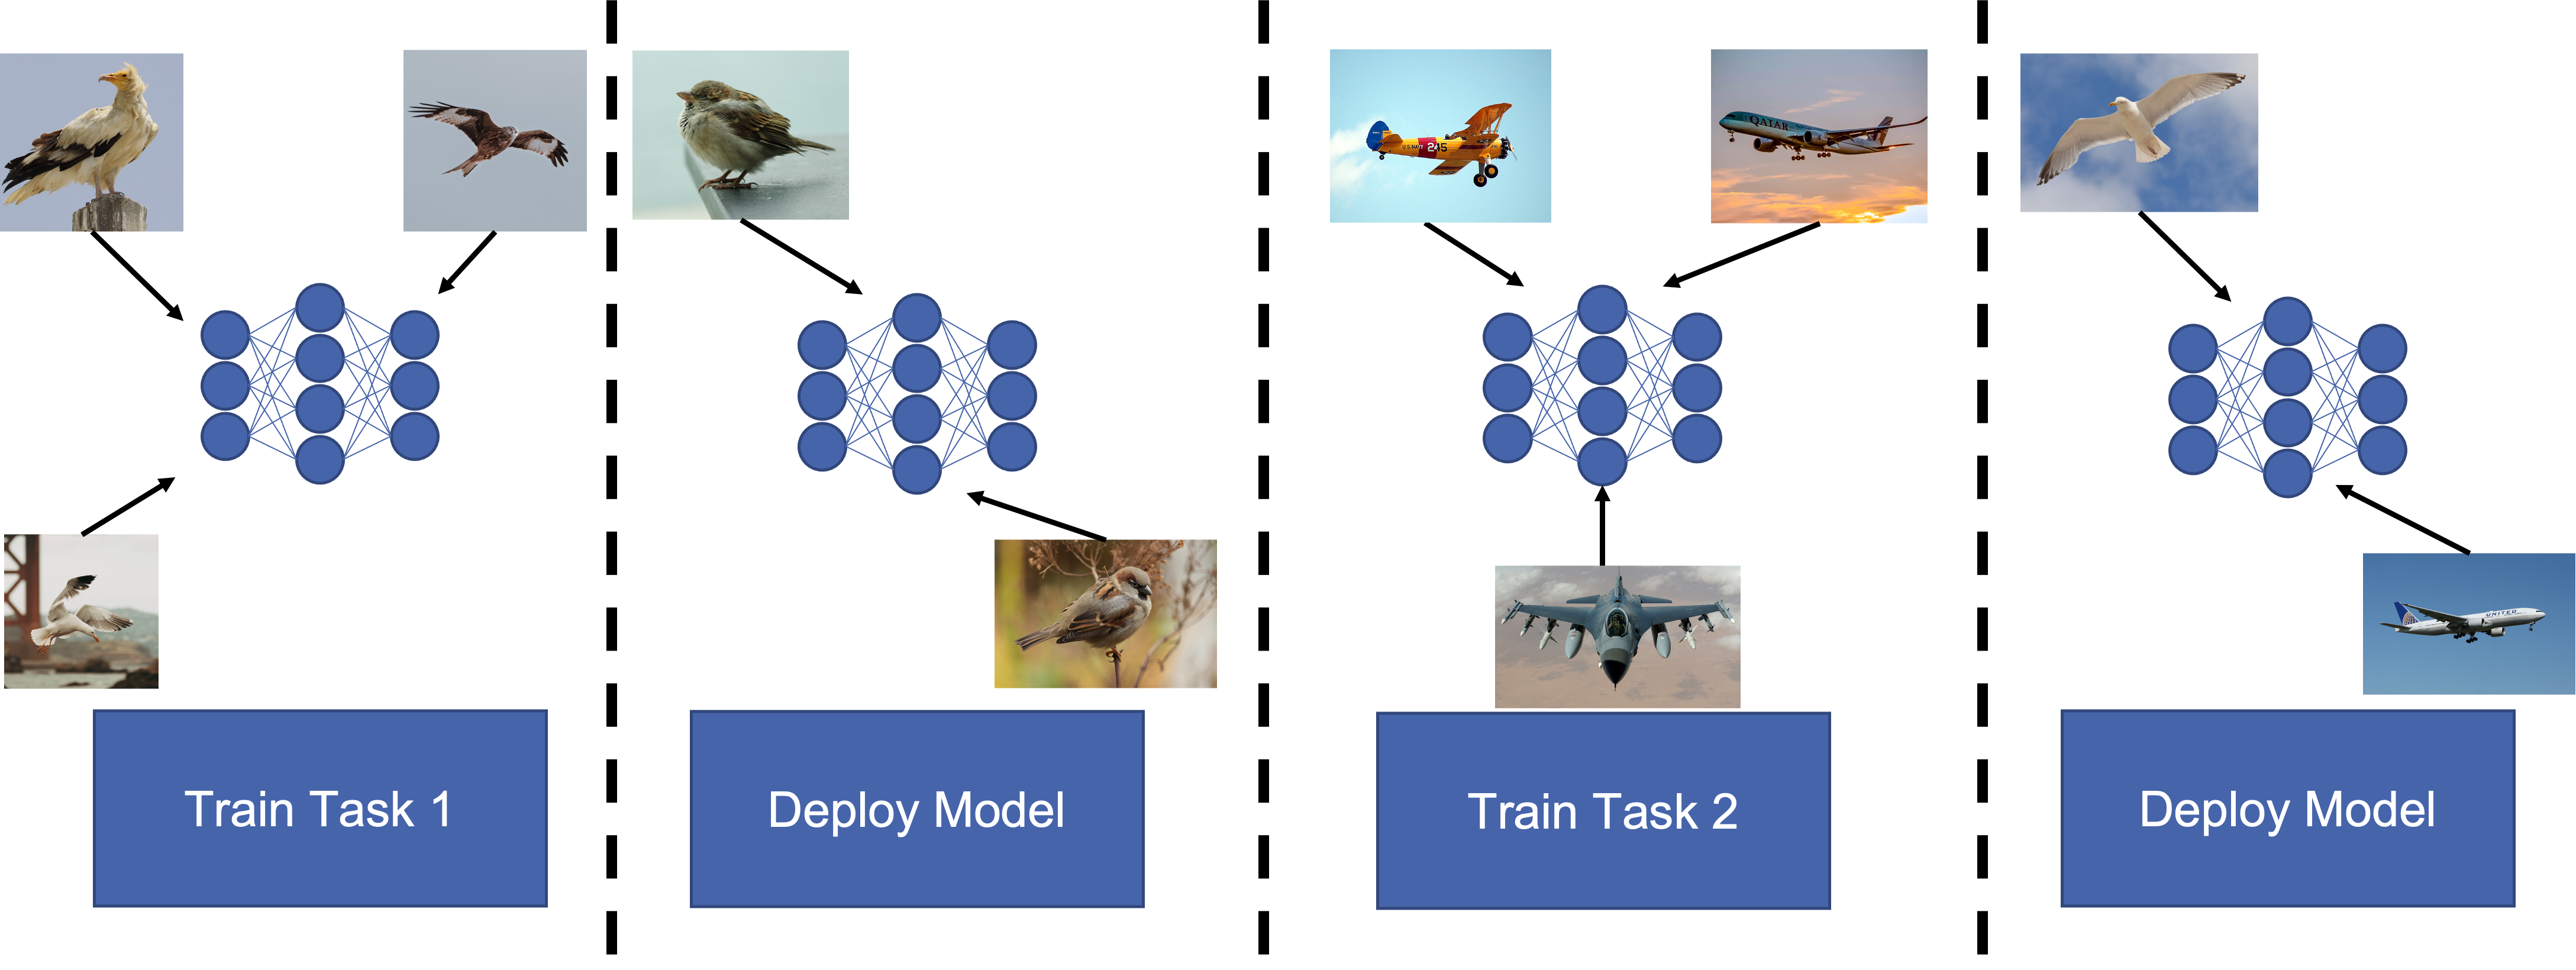
\includegraphics[width=.9\linewidth]{images/CL_workflow.png}
    \caption[Continual Learning Workflow]{Example for the classic Continual Learning Workflow. In this example, the model is first trained on different species of
    birds. It is then deployed to differentiate these species. Next, the model is trained on planes. After being deployed again, the model should now differentiate
    the planes as well as the birds.}
    \label{fig:CLWorkflow}
  \end{figure}

\subsection{The classic Active Learning Setting}
\label{sec:Methodology:ALSetting}
%Mention classic pool-based Active Learning setting, what batches are, contrast the continual
% learning setting, saying that the "tasks" are not independent

\subsection{Combining Continual and Active Learning}
% Mention the issues with the classic CL and AL setting, describe how synergising the two approaches
% can help overcome these issues and describe the approach in detail
\label{sec:Methodology:CombiningCLandAL}
The problem with classic Active Learning is that it is very resource intensive. When training a model using pool-based Active Learning on a dataset of size $n$,
with batch size $b$, the model will be trained $\frac{n}{b}$ times on the current labeled pool, equating to $\frac{n^2}{b} + n$ data points overall (we provide a
short derivation of this number in \ref{sec:appendix:FirstSection}). The problem with the number of data points used for training is that it is dependent on the
batch size $b$. While \cite{beck2021effective}When comparing this to the classic Continual Learning setting, where the model is trained
once using $n$ data points, it is clear to see that Active Learning comes with a considerable overhead. The overhead of Active Learning is even more pronounced
when considering the running time of the Active Learning Algorithms. For more details we refer to the TODO experimental sections.
\begin{algorithm}
    \caption{Pool-based Continual Active Learning} \label{alg:PoolBasedContinualActiveLearning}
    \begin{algorithmic}[1]
        \Require Unlabeled data $U$,Labeled data $L = \emptyset$:, Oracle $O$, Model $M$, budget $B$
        \State Select $k$ data points from $U$ at random, obtain labels by querying $O$ and set $L=\{x_1,\ldots,x_1\}$
        and $U = U \setminus \{x_1,\ldots,x_1\}$ \Comment{Initialization}
        \State Train $M$ on initial labeled set $L$
        \While{label budget $B$ not exhausted}
            \State Select $l$ data points from $U$ predicted to be the most informative by the Active Learning strategy
            \State Obtain labels $y_i,\ldots,y_l$ by querying $O$ for $x_i,\ldots,x_l$
            \State {\color{red} Train $M$ on current labeled batch $\{(x_iy_i),\ldots,(x_l,y_l)\}$}
            \State Set $L= L \cup \{x_i,\ldots,x_l\}$ and $U = U \setminus \{x_i,\ldots,x_l\}$
            \State Train $M$ on labeled set $L$
        \EndWhile
    \end{algorithmic}
\end{algorithm}

\section{Continual Active Learning for Model Stealing}
\label{sec:Analysis:SecondSection}
% Transition to model stealing and elaborate why the continual active learning approach is interesting
% in the model stealing domain. Explain how the continual active learning approach has to be modified
% to apply it to model stealing. Best use a figure similar to the figure explaining the CAL approach
% and highlight the parts that are different
\begin{figure}[ht]
    \centering
    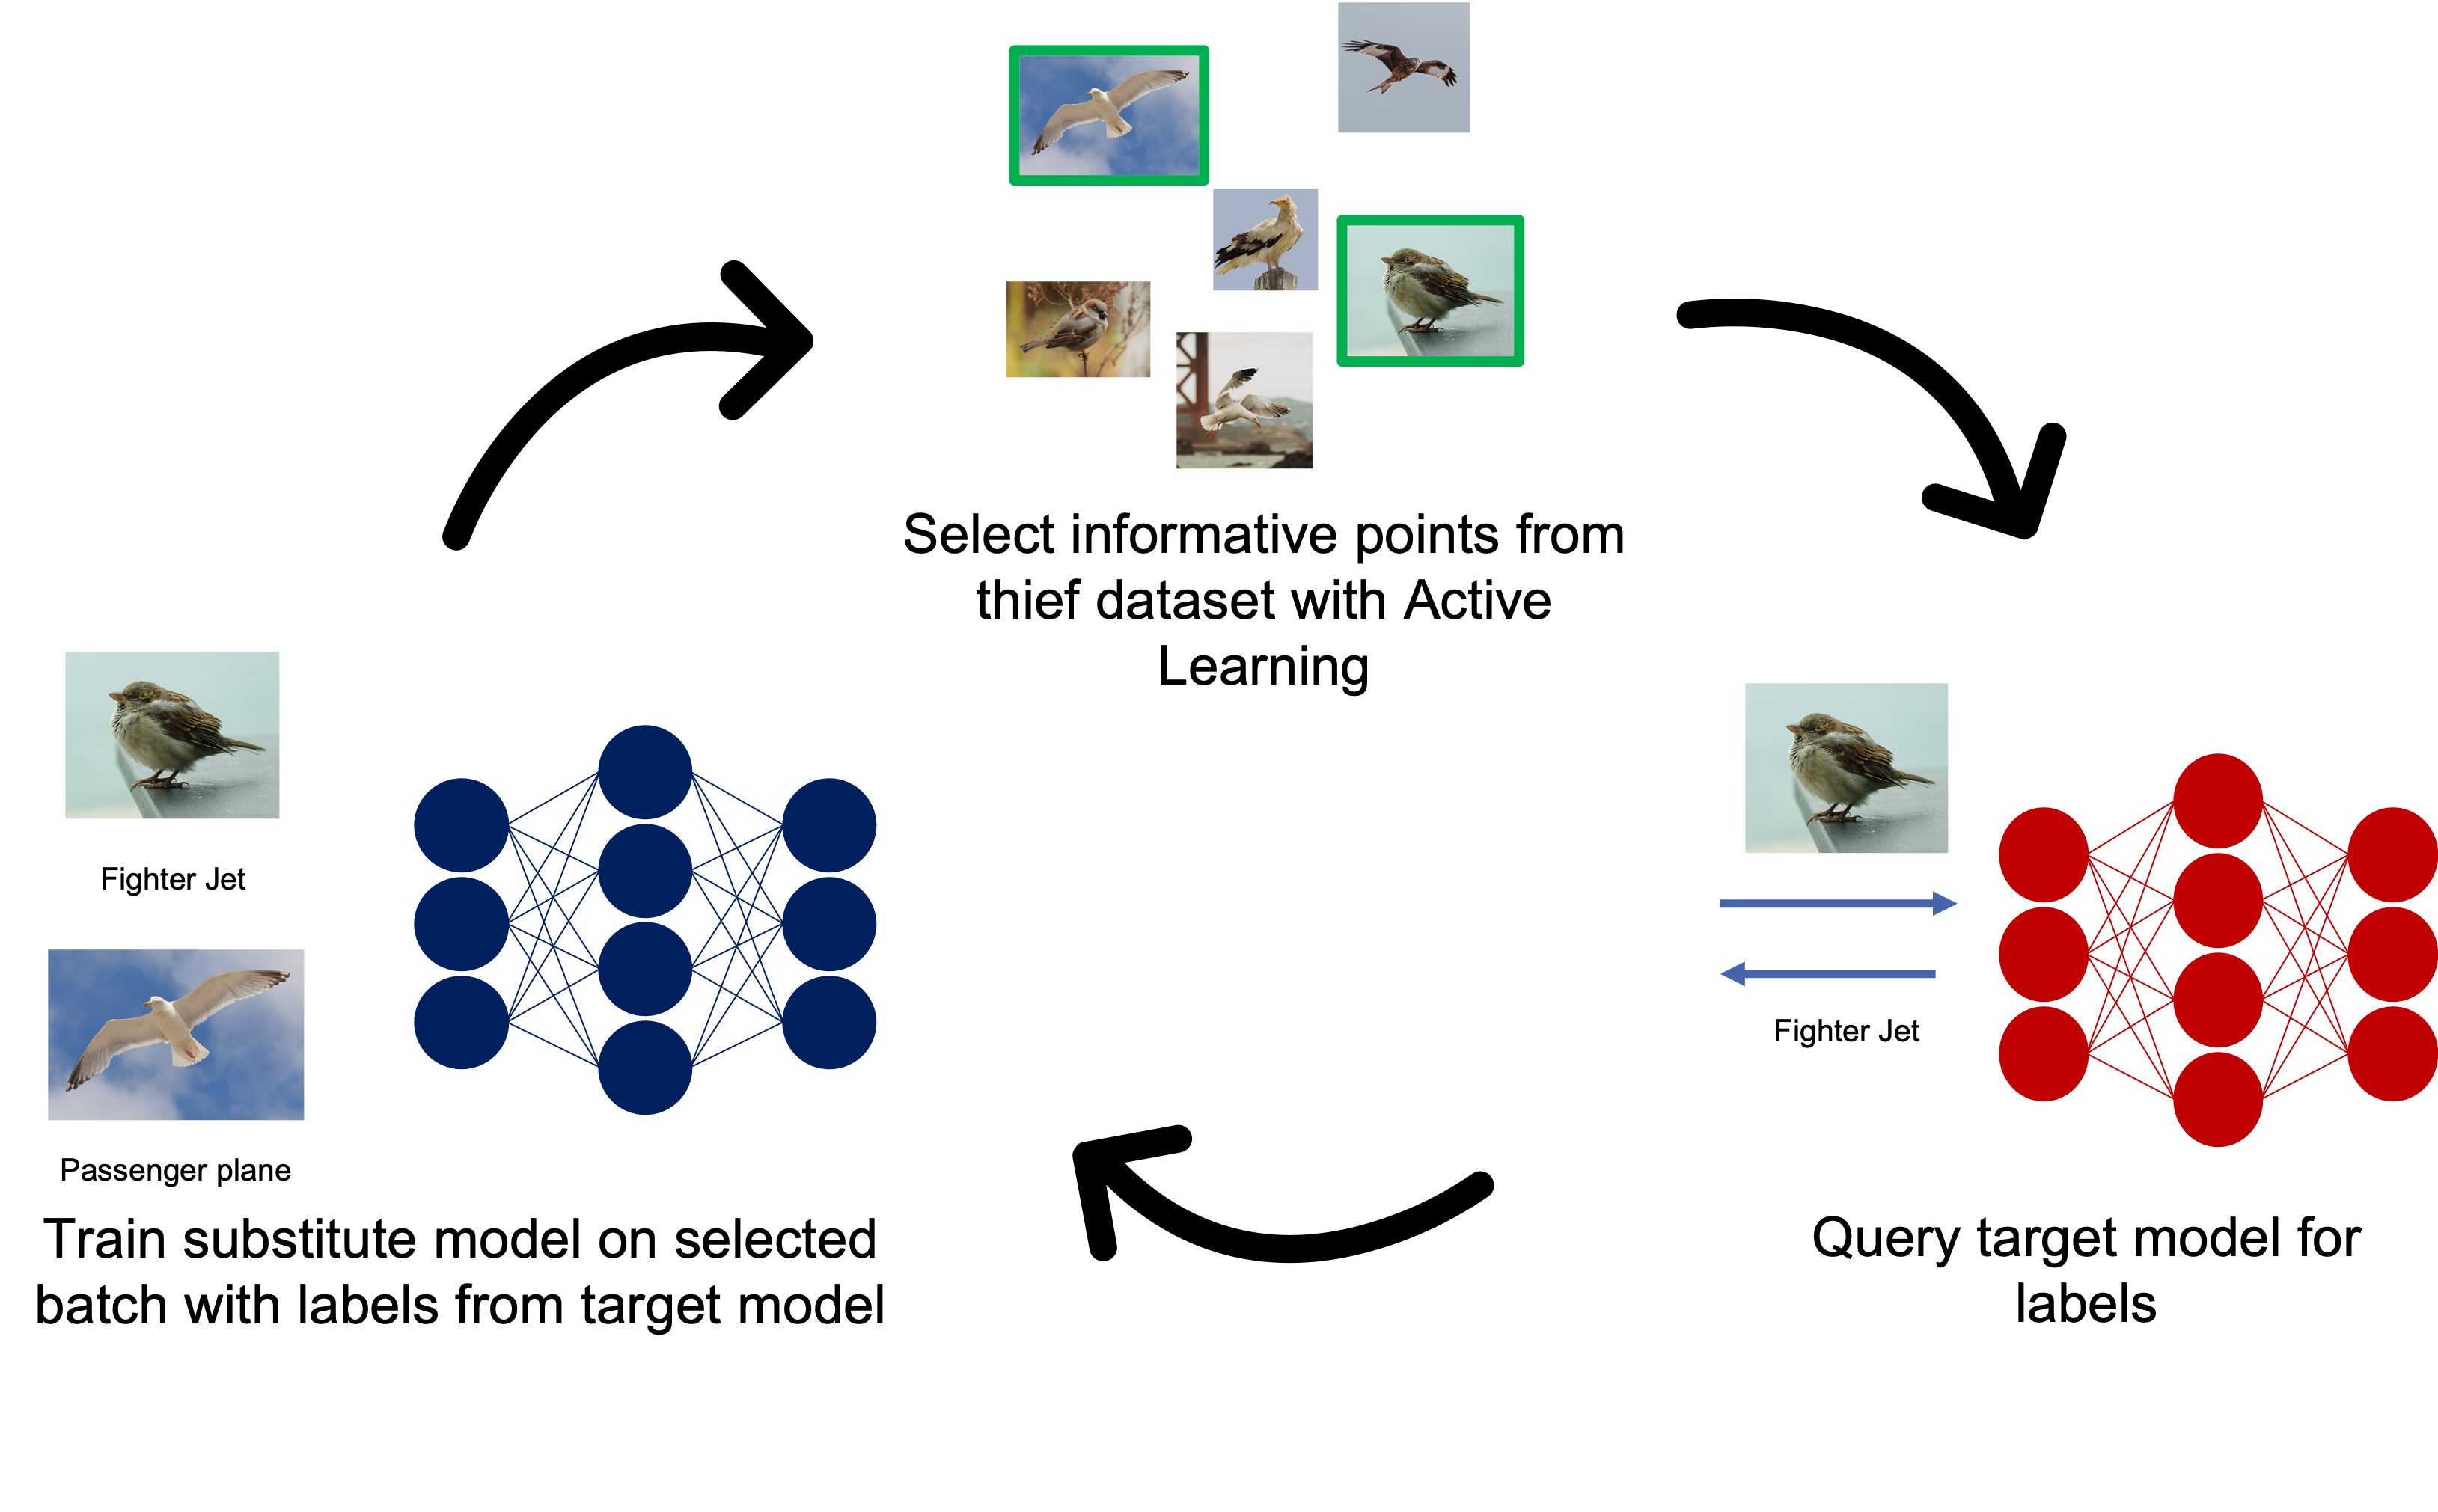
\includegraphics[width=.9\linewidth]{images/Calms_workflow.png}
    \caption[Continual Active Learning for Model Stealing Workflow]{Example of the Continual Active Learning for Model Stealing Workflow. In this example, the thief
    dataset consists of birds while the target model was trained to classify planes. In each iteration, a batch of informative samples is selected by the Active Learning
    strategy first. Next, the target model is queried for the labels of the selected samples. Since our thief dataset is composed of NNPD data, the associated labels have
    an incorrect semantic meaning. The thief model is then trained only on the selected samples from the current batch. This process is repeated iteratively.}
    \label{fig:CalmsWorkflow}
  \end{figure}

\section{Third Section}
\label{sec:Analysis:ThirdSection}

\dots
%% ---------------------
%% | / Example content |
%% ---------------------